% Licensed under the Creative Commons Attribution Share Alike 4.0 International.
% See the LICENSE file in the repository root for full license text.

\begin{problemset}
	\item 体验调试程序。在 Visual Studio 中使用“Windows 桌面向导”新建一个\textbf{空白的(勾选“空项目”复选框)}控制台应用程序项目,在其中新建一个空白源文件(扩展名为 \lstinline{.c}),然后在源文件中输入以下代码。

	\begin{lstlisting}[language=c, moreemph={[2]factorial}]
#include <stdio.h>

int factorial(int n)
{
	if (n == 0)
		return 1;
	int return_value = n * factorial(n - 1);
	return return_value;
}

int main()
{
	int result = factorial(3);
	printf("%d", result);
}
	\end{lstlisting}

	\begin{enumerate}
		\item 输入代码时,编辑器会触发代码自动补全功能,如图 \ref{pic:auto_complete} 所示。在你输入代码的过程中,你发现代码自动补全能帮你做哪些事?请做简要描述。

		\begin{figure}[H]
			\centering
			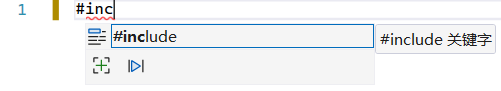
\includegraphics[width=0.6\linewidth]{pic/auto-complete.png}
			\caption{代码编辑器的代码自动补全功能}
			\label{pic:auto_complete}
		\end{figure}

		\item 根据输入代码时看到的英文单词以及数字,猜测这个程序的作用。

		\item 直接运行程序,程序会在控制台窗口中输出一个数。这个数是多少?你可以通过本小问验证上一小问的猜想。

		\item 在第 13 行处下断点,点击开始调试,然后不断逐语句调试,直到当前行为第 14 行,观察整个过程中当前行以及“调用堆栈”窗口的变化情况。当“调用堆栈”窗口中的函数发生变化\textbf{后}(如果仅仅是栈顶函数的当前行发生改变,则不予理会),记录“调用堆栈”窗口中的内容,并在\textbf{再一次点击“逐语句”后}通过“局部变量窗口”记录所有名为 \lstinline{n} 和 \lstinline{return_value} 的变量的值。

		提示:你应该总共记录 8 次。
	\end{enumerate}

	\item 创建非空白项目。在 Visual Studio 中使用“Windows 桌面向导”新建一个\textbf{桌面}应用程序项目,\textbf{并且不要勾选“空项目”复选框,其他复选框保持默认}。项目创建结束后,直接生成并调试。简要描述观察到的程序运行现象。

	\item 体验在线评测平台。几乎所有在线评测平台上的前几道题中都有一道名为 “A + B Problem” 的习题,用于测试在线评测平台是否正常工作以及帮助新手熟悉评测环境。在任一在线评测平台中找到\textbf{最靠前的} “A + B Problem”\footnote{有些难题也可能取名为 “A + B Problem”,那种题一般都不会出现在题库的最前面。},编写代码,通过此题。记录所有做题过程中在线评测平台反馈给你的结果。

	提示:“A + B Problem” 一般在题目中就附有标准答案。如果你看到的 “A + B Problem” 中没有标准答案,可以考虑换一个在线评测平台。
\end{problemset}